\chapter{Methodology}

This chapter contains a comprehensive description of the design of the proposed matching system, demonstrates how it addresses the problem, and justifies the design with the support of evaluation results.

The workflow of a typical ontology matching methodology is given in Figure \ref{fig:methodology}. The central part, being "selecting and composing matchers", is the stage that should be put most effort on.

\begin{figure}[ht]
\begin{center}
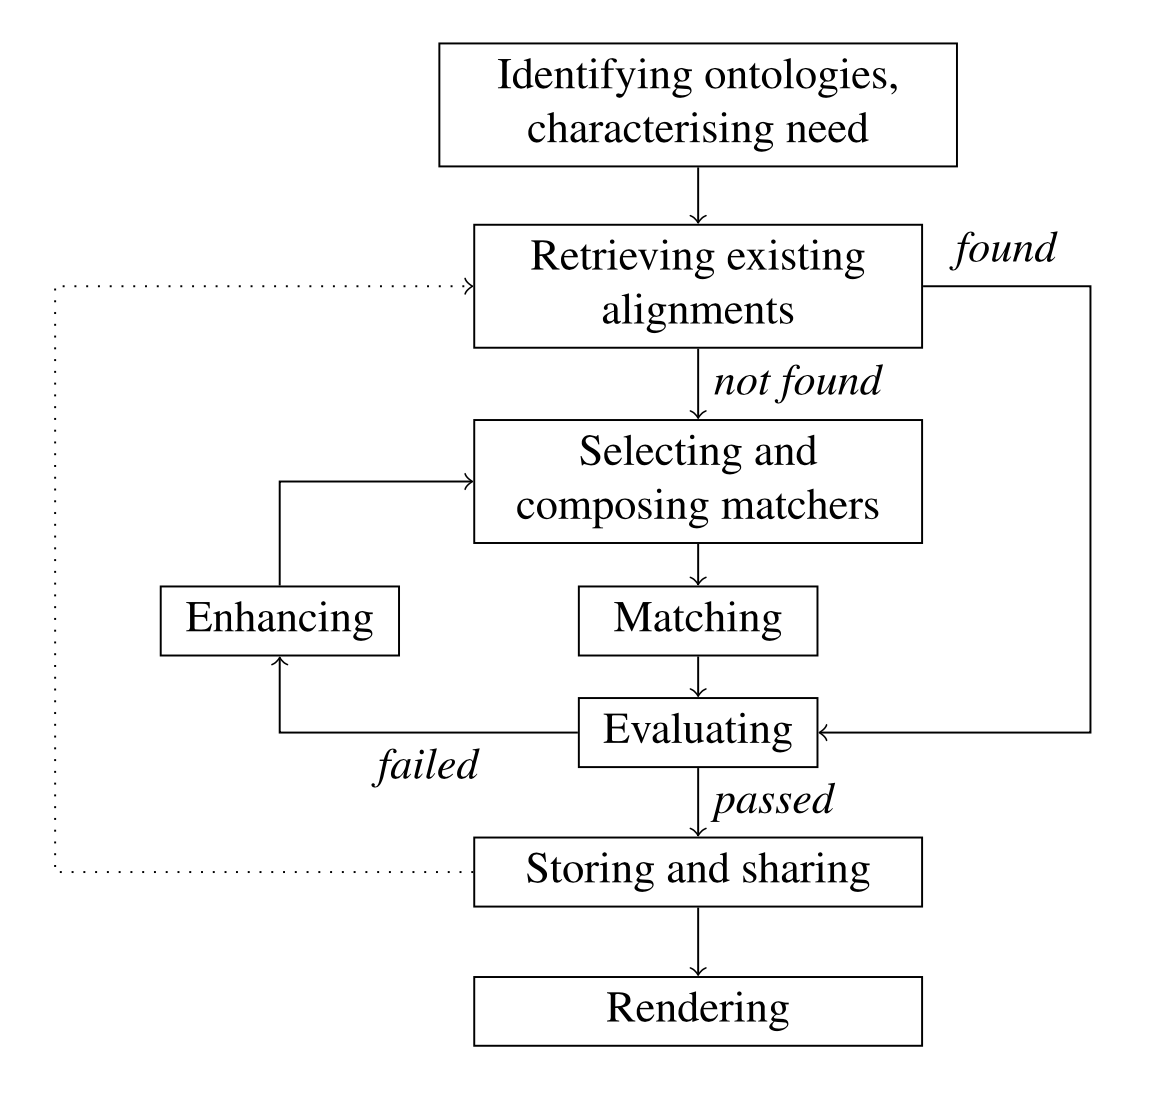
\includegraphics[width=0.4\textwidth]{img/methodology.png}
\caption{The matching methodology workflow}
\label{fig:methodology}
\end{center}
\end{figure}

According to the structures of existing popular systems and the evaluation results provided in the previous chapter, the structures of three systems, namely Lily, LogMap and PARIS, are the ones decided to be focused on. Lily has shown excellent performance in the SPIMBENCH instance matching tracks, with not only high precision, F-measure and recall rate, but also a reasonable time efficiency. LogMap was designed to be able to deal with large-scaled ontologies in general purposes, which suits the need of matching enormous instances in data integration. PARIS, being a probability-based system, deals with not only classes and instances, but also tries to align relations. This can be used as an ideal start of the project, the fundamental aim of which being investigating the aid of matching object relations in instance matching. Based on the common points of their structures, the following design selects methodological components to be used and propose a basic structure of integrating them.

\begin{spacing}{1.2}
\begin{enumerate}
	\item The components in the input ontologies, including not only classes and instances, but also object properties, data properties, values and relation roles between different instances, are interpreted as strings.
	\item String-based techniques such as Levenshtein Distance and lexical indexing are then used to discover their syntactical similarities.
	\item Public general-purpose dictionaries such as WordNet may be considered for the semantic evaluation of the strings.
	\item A preliminary match between the corresponding entities is performed, where the alignments with highest confidence are kept.
	\item Based on the existing matches available, description logic reasoners are exploited for the inference of nontrivial relations.
	\item Structure-based techniques such as similarity flooding are adopted to determine the matching instances by checking the similarity between their adjacently related instances.
	\item Description logic reasoners are used for a systematic discovery of inconsistencies based on the matching instances and logical relations. Pruning will be carried out if inconsistencies are identified.
\end{enumerate}
\end{spacing}

It should be noted that although these are the proposed algorithmic components are currently decided as suitable for the general purpose instance matching, the selection and combinational order of them is subject to changes and required more detailed design. Further knowledge about the linkage of those components in existing systems should be acquired, which is the current and next stage of this project.

\chapter{Implementation}

% This chapter contains a comprehensive description of the implementation of your software, including the language(s) and platform chosen, problems encountered, any changes made to the design as a result of the implementation, etc.

% Explaining how your software was tested (using different datasets or in different environments), statistical evaluation of performance, results of user evaluation questionnaires, etc.

For the implementation of the proposed instance matching system, Java will be used as the primary programming language, as the supplementary APIs and evaluation initiatives use Java officially. This chapter introduces some core Java classes and functions from the APIs and SDKs that will be used in the implementation.

\section{Development}

\subsection{OWL API}

In order to perform basic manipulation over the entities in OWL 2 ontologies, the \\
\texttt{org.semanticweb.owlapi.model} package should be utilised. Specifically, classes like \texttt{AddAxiom}, \texttt{AddImport}, \texttt{AddOntologyAnnotation} and their corresponding removers are the fundamental operations that will be used along.
\\\\
Parser and renderer classes are available for various OWL 2 syntaxes, including the OWL/XML, RDF/XML, DL, functional, Manchester and Turtle, in their respective packages. The \texttt{parse} and \texttt{render} function can be used to read from one syntax and then write into another. These can be useful when another desired software tool or API have support issues with specific syntaxes.
\\\\
Classes inside the package \texttt{org.semanticweb.owlapi.profiles} can be used to check whether an input ontology falls into a certain OWL 2 profile. This helps in analysing the reasonability and decidability for tasks provided in the evaluation framework.
\\\\
The \texttt{org.semanticweb.owlapi.vocab} package contains \texttt{Enum} classes, such as \\
\texttt{BuiltInVocabulary}, \texttt{Namespaces} and \texttt{OWL2Datatype}, that enumerate various kinds of OWL 2 vocabularies. These are useful for custom construction and interpretation of expressions.
\\\\
While the implementation does not build a reasoner for itself, the package \\
\texttt{org.semanticweb.owlapi.reasoner} is required for the reasoner APIs to be based on.

\subsection{Reasoner API}

While different reasoners have different usages, their core components and functionalities are similar. Take the HermiT reasoner for example, the \texttt{org.semanticweb.HermiT.model} package contains class definitions for logical models such as equality, inequality, role, inverse role, atomic concept, atomic role, and so on, while the \\
\texttt{org.semanticweb.HermiT.structural} package contains classes that manages the structure of built-in properties and axioms.

\subsection{Alignment API}

For the basic use of Alignment API, the package \texttt{fr.inrialpes.exmo.align.parser} is sufficient for the parsing of alignment syntax. The API also provides a WordNet-based implementation besides the basic implementation.

\subsection{SPARQL-Generate API}

The \texttt{fr.mines\_stetienne.ci.sparql\_generate.query} package in SPARQL-Generate API contains the model for SPARQL queries, which is used for query construction. The package \texttt{fr.mines\_stetienne.ci.sparql\_generate.engine} can then be used to execute the query using one of the \texttt{exec} methods in its classes.

\section{Evaluation}

In order to evaluate the instance matching results, the implementation needs to be wrapped in the HOBBIT evaluation framework \cite{}. HOBBIT has provided a library called the HOBBIT Java SDK to simplify the wrapping as well as local testing with supported data. In order to use the SDK, the Maven environment should be set up properly according to \url{https://hobbit-project.github.io/java_components}. Then the components of a benchmark should be made to implement the \texttt{org.hobbit.core.components.Component} interface. The details of system adapter development and benchmark components should be investigated into details.
